\documentclass[a4paper,12pt]{article}
\usepackage[russian]{babel}
\usepackage[T2A]{fontenc}
\usepackage[utf8]{inputenc}
\usepackage{geometry}
\usepackage{amsmath}
\usepackage{graphicx}
\usepackage{cancel}
\usepackage{float} 
\usepackage{xcolor}
\usepackage{array}
\usepackage{caption}
\usepackage{booktabs}
\usepackage{amssymb}
\usepackage{subcaption}
\usepackage{pgfplots}
\pgfplotsset{compat=1.18}
\usetikzlibrary{arrows.meta, matrix}
\usepackage{capt-of}
\usepackage{multirow}
\usepackage[siunitx]{circuitikz}
\usepackage[bottom]{footmisc}
\usepackage{tcolorbox}
\usepackage{nicematrix}
\usepackage{tikz}
\usetikzlibrary{positioning, arrows.meta}

% --- hyperref ОДИН РАЗ ---
\usepackage{hyperref}
\hypersetup{linktoc=page}
\hypersetup{
	colorlinks=true,
	linkcolor=red,
	citecolor=red,
	urlcolor=red,
	filecolor=red,
}

% --- Содержание ---
\usepackage{tocloft}
\usepackage{etoolbox}
\usepackage{hyperref}
\hypersetup{
	colorlinks=true,
	linkcolor=red,
	citecolor=red,
	urlcolor=red,
}

% Патчим \tableofcontents: текст строк — без ссылок и чёрный
% Это делается через замену \contentsline внутри TOC
\preto\tableofcontents{%
	\begingroup
	% Переопределяем contentsline так, чтобы текст был чёрным без ссылки,
	% а номер страницы — красной ссылкой
	\renewcommand{\contentsline}[4]{%
		\ifnum\pdfstrcmp{##1}{section}=0
		\vskip 4pt{\normalfont\color{black}##2}\nobreak\hfill
		{\normalfont\color{red}\hyperlink{##4}{##3}}\par
		\else\ifnum\pdfstrcmp{##1}{subsection}=0
		\vskip 2pt\hspace{1.5em}{\normalfont\color{black}##2}\nobreak\hfill
		{\normalfont\color{red}\hyperlink{##4}{##3}}\par
		\else
		\vskip 1pt\hspace{3em}{\normalfont\color{black}##2}\nobreak\hfill
		{\normalfont\color{red}\hyperlink{##4}{##3}}\par
		\fi\fi
	}%
}
\appto\tableofcontents{\endgroup}

\newcommand{\figwidth}{0.7\textwidth}

% tocloft — только для отступов, без переопределения шрифтов
\usepackage{tocloft}

% --- Листинги ---
\usepackage{listings}

\definecolor{codebg}{RGB}{250,250,252}
\definecolor{linenumcolor}{RGB}{150,150,170}
\definecolor{mathblue}{RGB}{30,100,200}
\definecolor{mathorange}{RGB}{200,100,20}
\definecolor{matlabblue}{RGB}{0,0,200}
\definecolor{matlabgreen}{RGB}{30,130,30}
\definecolor{matlaborange}{RGB}{200,80,0}

\lstdefinelanguage{Mathematica}{
	keywords={Plot, Eigenvalues, MatrixExp, RiccatiSolve, IdentityMatrix,
		Inverse, Transpose, Simplify, Eigensystem, StateSpaceModel,
		ControllabilityMatrix, MatrixRank, Export, FileNameJoin,
		NotebookDirectory, ConstantArray, ZeroMatrix, NDSolve,
		Evaluate, LineLegend, Placed, Directive, Opacity, Filling,
		FillingStyle, PlotStyle, PlotLegends, PlotRange, Frame,
		Axes, FrameLabel, GridLines, GridLinesStyle, AspectRatio,
		Style, FontFamily, FontSize, Thick, Dashed, Dotted,
		DotDashed, RGBColor, GrayLevel, LegendLayout, LabelStyle,
		Subscript, Table, Do, Module, Block, If, True, False, Automatic},
	sensitive=true,
	morecomment=[s]{(*}{*)},
	morestring=[b]",
}

\lstdefinestyle{mma}{
	language=Mathematica,
	basicstyle=\ttfamily\small,
	keywordstyle=\color{mathblue}\bfseries,
	commentstyle=\color{linenumcolor}\itshape,
	stringstyle=\color{mathorange},
	numberstyle=\tiny\color{linenumcolor},
	numbers=left,
	numbersep=10pt,
	backgroundcolor=\color{codebg},
	frame=single,
	frameround=tttt,
	framesep=4pt,
	rulecolor=\color{mathblue!40},
	breaklines=true,
	tabsize=4,
	showstringspaces=false,
	captionpos=b,
	xleftmargin=15pt,
	xrightmargin=5pt,
}

\lstdefinestyle{matlab}{
	language=Matlab,
	basicstyle=\ttfamily\small,
	keywordstyle=\color{matlabblue}\bfseries,
	commentstyle=\color{matlabgreen}\itshape,
	stringstyle=\color{matlaborange},
	numberstyle=\tiny\color{linenumcolor},
	numbers=left,
	numbersep=10pt,
	backgroundcolor=\color{codebg},
	frame=single,
	frameround=tttt,
	framesep=4pt,
	rulecolor=\color{matlabblue!30},
	breaklines=true,
	tabsize=4,
	showstringspaces=false,
	captionpos=b,
	xleftmargin=15pt,
	xrightmargin=5pt,
	escapeinside={\%*}{*)},
	morekeywords={cvx_begin,cvx_end,sdp,variable,minimize,maximize},
}

\lstset{style=mma}

\renewcommand{\lstlistingname}{Листинг}
\DeclareCaptionFormat{redlisting}{#1\textcolor{red}{#2}#3}
\captionsetup[lstlisting]{format=redlisting}

\geometry{left=1.5cm, right=2cm, bottom=2cm, top=2cm}
\captionsetup[figure]{name=Рисунок}
\captionsetup[table]{name=Таблица}
\captionsetup{labelsep=endash}


\begin{document}
	
	\begin{titlepage}
		\centering
		
		\vspace*{0.5cm}
		{\small
			Министерство науки и высшего образования Российской Федерации\\[2pt]
			Федеральное государственное автономное образовательное учреждение\\
			высшего образования\\[2pt]
			\textbf{«Национальный исследовательский университет ИТМО»}\\
		}
		
		\vspace{0.8cm}
		\hrule height 0.8pt
		\vspace{0.3cm}
		
		{\large Факультет систем управления и робототехники}
		
		\vspace{0.3cm}
		\hrule height 0.4pt
		\vspace{2.5cm}
		
		{\Huge\bfseries ОТЧЁТ}\\[0.4cm]
		{\LARGE\bfseries о лабораторной работе №3}\\[0.8cm]
		
		\begin{tcolorbox}[
			colback=gray!4,
			colframe=gray!10,
			boxrule=0.8pt,
			arc=4pt,
			left=12pt, right=12pt, top=8pt, bottom=8pt
			]
			\centering
			{\large По дисциплине:\\[4pt]}
			{\large\bfseries «Основы цифрового производства»}\\[10pt]
			{\large Тема:\\[4pt]}
			{\large\bfseries «Программирование роботов»} \\[10pt]
			{\large Вариант: 1}
		\end{tcolorbox}
		\vspace{3cm}
		
		
		\begin{minipage}{0.45\textwidth}
			\raggedright
			{\large\bfseries Студенты:}\\[4pt]
			\textit{Кокорин Александр 470170}\\
			\textit{Охрименко Ева 409290}\\
			\textit{Медвеженкова Марина 409114}
		\end{minipage}%
		\hfill
		\begin{minipage}{0.45\textwidth}
			\raggedleft
			{\large\bfseries Преподаватель:}\\[4pt]
			\textit{Университет ИТМО \hfill Киприянов Кирилл Васильевич
			}
		\end{minipage}
		
		\vfill
		\vspace{0.4cm}
		{\large Санкт-Петербург, 2026}
	\end{titlepage}
	
	
	
\section{Алгоритм управления}
Программа \texttt{change} реализует последовательный перенос двух объектов (Part 1, Part 2) со стеллажа на стол. Логика работы построена по принципу «подход -- захват -- перенос -- укладка -- отход».

Для каждой детали $i \in \{1, 2\}$ выполняется следующий цикл:
\begin{enumerate}
	\item \texttt{MoveJ (HOME)} -- переход в безопасную исходную позицию.
	\item \texttt{MoveJ (part$i$ near)} -- быстрый подход к зоне захвата на стеллаже.
	\item \texttt{MoveJ (part$i$)} -- точное позиционирование захвата над деталью.
	\item \texttt{Attach} -- активация захвата OnRobot SG-b.
	\item \texttt{MoveJ (HOME)} -- возврат в безопасную зону для обхода препятствий.
	\item \texttt{MoveJ (targ$i$)} -- перемещение к точке укладки на столе.
	\item \texttt{Detach} -- отпускание детали.
	\item \texttt{MoveJ (HOME)} -- завершение цикла, возврат в исходную точку.
\end{enumerate}

Использование промежуточной точки \texttt{HOME} между захватом и укладкой обеспечивает бесконфликтную траекторию движения робота вокруг стеллажа. Точка была добавлена в качестве отладки программы, так как были обнаружены коллизии.

\section{Иллюстрации процесса работы}

На рисунках ниже представлены ключевые этапы выполнения управляющей программы \texttt{change} в среде RoboDK.

\begin{figure}[H]
	\centering
	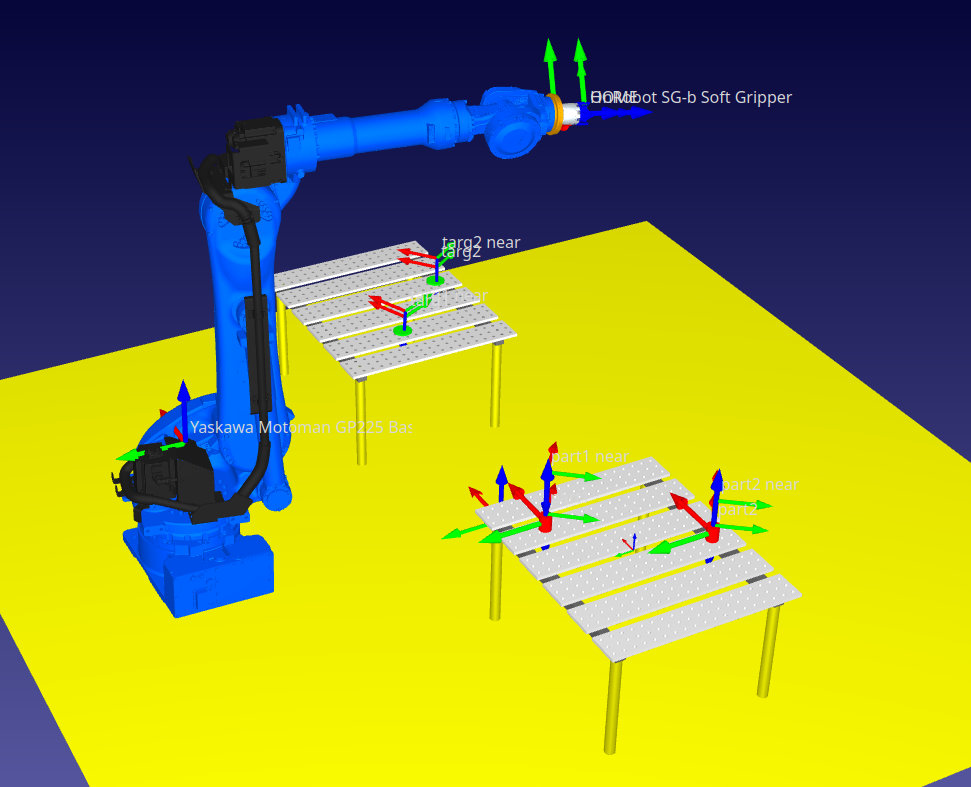
\includegraphics[width=0.6\textwidth]{../images/scene_start.png}
	\caption{Общая сцена: начальное состояние рабочей ячейки. Робот Yaskawa GP225 находится в позиции HOME, детали Part 1 и Part 2 расположены на стеллаже Source rack}
\end{figure}

\begin{figure}[H]
	\centering
	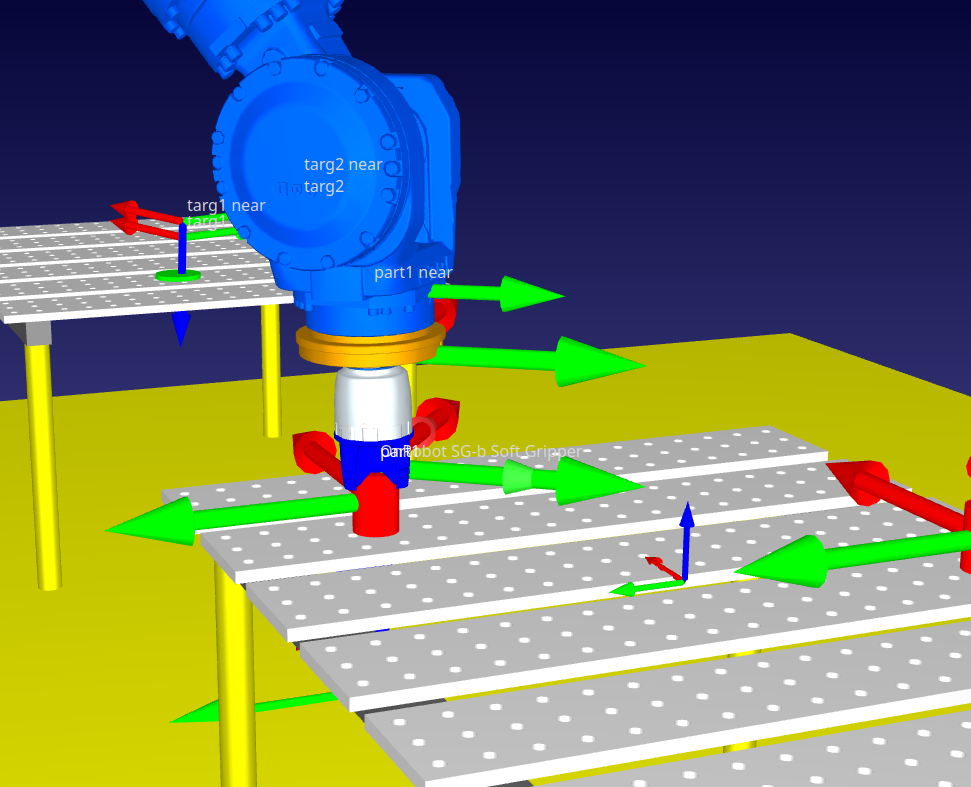
\includegraphics[width=0.6\textwidth]{../images/grasp_moment.png}
	\caption{Момент захвата: инструмент OnRobot SG-b фиксирует деталь Part 1 в точке part1. Траектория подхода обеспечивает отсутствие коллизий со стеллажом}
\end{figure}

\begin{figure}[H]
	\centering
	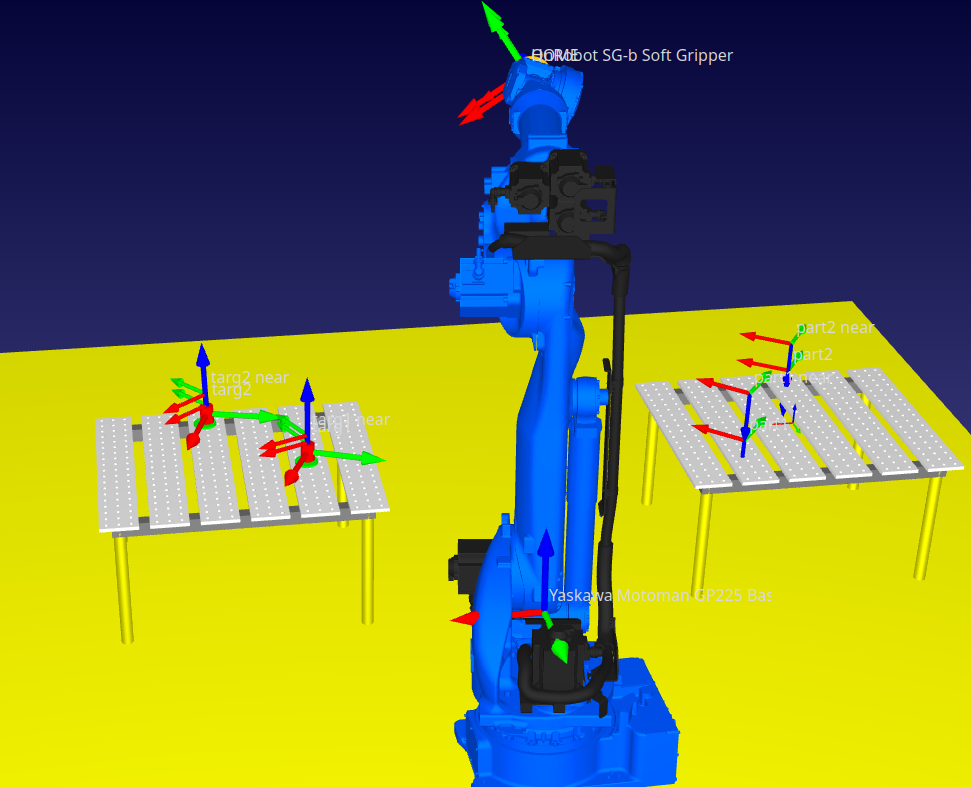
\includegraphics[width=0.6\textwidth]{../images/work_result.png}
	\caption{Результат работы: обе детали успешно перемещены на стол Destination table в целевые точки Target 1 и Target 2. Программа выполнена без ошибок}
\end{figure}







	
\end{document}